\section{Evaluation}
\label{sec:evaluation}
\label{sec:benchmark}

We evaluated our approach by implementing a variety of real-life
applications including:
\begin{itemize}
\item \emph{Numerical Differentiation} with the Savitsky-Golay
  smoothing filter, a scientific application used to compute the
  derivative of a function when its analytical form is not available
  (e.g. on large experimental data);
\item \emph{Black Scholes Option
  Pricing}, a financial application for pricing European
options\footnote{financial instruments that allow the owner to buy or
  sell the underlying asset at a fixed point in the future};
\item \emph{Ad Prediction}, a Bayesian inference application for
predicting the rate at which ads are clicked on by users of Microsoft
Bing.
\end{itemize}
However, due to lack of space, we focus on \emph{Reverse Time
  Migration} (RTM), the most complex application in our suite. RTM is
a seismic imaging application used to detect geological structures,
based on the Earth's response to injected acoustic waves. We used
\FAST{} to implement the dataflow kernels for the memory controllers
and the computational kernel. We used the design space exploration
aspect description of Listing \ref{lst:aspect-exploration} to analyse
trade-offs between accuracy and resource usage (Figure~3.a) and
identify resource bottlenecks (Figure~3.b). This shows that simple
aspect descriptions can be used effectively to identify
counter-intuitive results (e.g. large savings in DSP usage achieved
when decreasing mantissa from 24 to 22 bits). The automated process
also improves design portability, allowing optimisations to be
explored on different platforms without manual intervention.

\begin{figure}[!ht]
\centering
\makebox[\textwidth][c]{%
\subfloat[]{%
  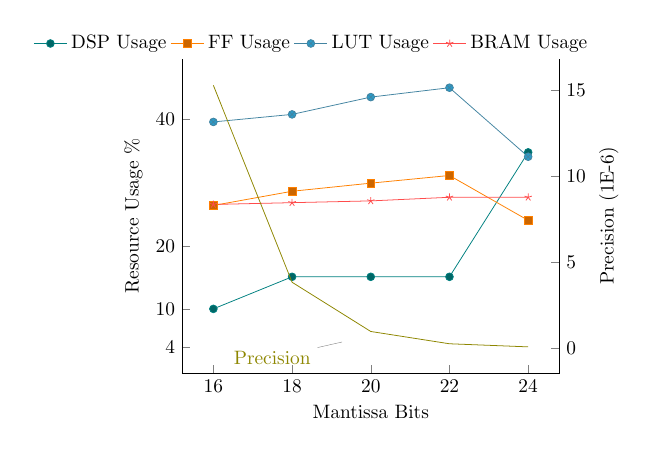
\begin{tikzpicture}[scale=0.7]
    \begin{axis}[
      cycle list name=exotic,
      ymin=0,
      axis y line*=left,
      axis x line*=bottom,
      xlabel=Mantissa Bits,
      ylabel=Resource Usage \%,
      xtick=data,
      ytick={4, 10, 20, 40, 50, 70, 80, 100},
      legend columns=4,
      legend entries={
        DSP Usage,
        FF Usage,
        LUT Usage,
        BRAM Usage},
      legend style={
        draw=none,
        anchor=east,
        at={(1.1, 1.05)}
      }
      ]
      \addplot coordinates {
        (24, 34.82)
        (22, 15.18)
        (20, 15.18)
        (18, 15.18)
        (16, 10.12)
      };
      \addplot coordinates {
        (24, 24.09)
        (22, 31.17)
        (20, 29.96)
        (18, 28.68)
        (16, 26.44)
      };
      \addplot coordinates {
        (24, 34.13)
        (22, 45.02)
        (20, 43.54)
        (18, 40.81)
        (16, 39.62)
      };
      \addplot coordinates {
        (24, 27.73)
        (22, 27.73)
        (20, 27.16)
        (18, 26.88)
        (16, 26.60)
      };
    \end{axis}
    \begin{axis}[
      ylabel=Precision (1E-6),
      axis y line*=right,
      axis x line=none,
      ]
      \addplot[color=olive] coordinates {
        (16, 15.2585)
        (18, 3.8146)
        (20, 0.9536)
        (22, 0.2394)
        (24, 0.0596)
      } node [pos=0.8,pin={190:Precision},inner sep=20pt] {};
    \end{axis}
  \end{tikzpicture}}\quad
\subfloat[]{%
  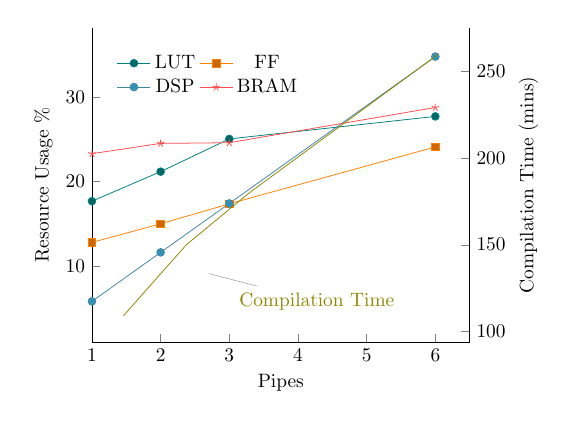
\begin{tikzpicture}[scale=0.7]
    \begin{axis}[
      cycle list name=exotic,
      xmin=1,
      ymin=1,
      xlabel=Pipes,
      ylabel=Resource Usage \%,
      axis x line* =bottom,
      axis y line* = left,
      legend columns=2,
      legend entries={
        LUT,
        FF,
        DSP,
        BRAM,
      },
      legend style={
        draw=none,
        at={(0.05,0.85) },
        anchor=west
      }
      ]
      \addplot coordinates {
        (1, 17.68)
        (2, 21.18)
        (3, 25.06)
        (6, 27.73)
      };
      \addplot coordinates {
        (1, 12.79)
        (2, 15.00)
        (3, 17.37)
        (6, 24.11)
      };
      \addplot coordinates {
        (1, 5.80)
        (2, 11.61)
        (3, 17.41)
        (6, 34.82)
      };
      \addplot coordinates {
        (1, 23.31)
        (2, 24.53)
        (3, 24.61)
        (6, 28.79)
      };
    \end{axis}
    \begin{axis}[
      ylabel=Compilation Time (mins),
      axis y line*=right,
      axis x line=none,
      ]
      \addplot[color=olive] coordinates {
        (1, 109)
        (2, 150)
        (3, 180)
        (6, 260)
      }  node [pos=0.2,pin={340:Compilation Time},inner sep=20pt] {};
    \end{axis}
  \end{tikzpicture}}
}
\caption[]{\emph{(a)} Exploration of accuracy versus resource usage
  trade-offs using the aspect description of
  \Cref{lst:aspect-exploration} and \emph{(b)} increase in compilation
  time and resource usage with number of parallel cores, used to
  identify design bottlenecks (limited resources which negatively
  impact design scalability).}
\label{g:nognot}
\end{figure}


\Cref{sec:appendix}, \Cref{table:rtm-performance} compares \FAST{}
implementations with other published results, showing that we
significantly outperform CPU implementations in terms of energy
efficiency (by a factor of 147.1) and performance (by a factor of
101.3) and match the performance of state-of-the-art manually
implemented FPGA designs. Other results from our benchmark suite
(summarised in \Cref{sec:appendix}, \Cref{table:benchmark}) show that
we can significantly reduce the number of API calls (by a factor of up
to 16) and lines of code required (by up to 60\%) while maintaining
performance when compared to manually developed dataflow designs for a
wider range of applications.
